\newpage

\section{Caso de estudio 1, $R_i=50[\Omega]$}

\subsection{Diseño de la etapa.}
\onehalfspacing
Entre los requisitos de diseño mencionados se solicita que la impedancia de entrada no cargue a la fuente, que se trabaje con resistencias menores a $1[M\Omega]$ y que la ganancia para cada fuente sea de $30$ veces.
\paragraph{}
A partir de dichas especificaciones se obtiene:
\begin{equation}
    \nonumber
    R_i=50[\Omega] \longrightarrow Z_{i1,2} \geq 10R_i
\end{equation}
donde $Z_{i1,2} = R$.
\paragraph{}
Tomando $R=1[k\Omega]$ y recordando que $A_{v1,2}(0)=30$
\begin{equation}
    \nonumber
    \frac{R_f}{R}=30 \longrightarrow R_f=30[k\Omega]
\end{equation}

\subsection{Cálculo de errores.}
\onehalfspacing
A partir de las carcterísticas eléctricas del $LM324$ se calculan los respectivos errores.

\subsubsection{Errores en DC.}
\onehalfspacing
\begin{equation}
    \nonumber
    \Delta V_{O}(v_{os}) = \left(1+2\frac{R_f}{R}\right) \cdot v_{os} = 61v_{os} = 61\cdot 2[mV]  = 122[mV]
\end{equation}
\begin{equation}
    \nonumber
    \Delta V_{O}(I_{os}) = -R_f\cdot I_p^{-} = 30[k\Omega]\cdot I_p^{-} = 30[k\Omega]\cdot 45[\mu A]  = 1350[\mu V]
\end{equation}
\begin{equation}
    \nonumber
    \Delta V_{O}(A_d<\infty) = \frac{FS}{T_O} = \frac{10[V]}{1640} = 6.1[mV]
\end{equation}
\begin{equation}
    \nonumber
    \Delta V_{O}(RRMC<\infty) = 0[V]
\end{equation}

\subsubsection{Errores en AC.}
\onehalfspacing
\textbf{Ancho de banda de plena potencia.} 
\paragraph{}
\begin{equation}
    \nonumber
    f_{HP} = \frac{SR}{2\pi \cdot V_{pp}} =  \frac{0.5\left[ \frac{V}{uS} \right]}{2\pi \cdot 10[V]} = 8[kHz]
\end{equation}

\paragraph{}
\textbf{Ancho de banda de pequeña señal.} 
\paragraph{}
\begin{equation}
    \nonumber
    f_{HP} = k\cdot f_T = \frac{R}{R+2R_f}\cdot f_T = 16.4[kHz]
\end{equation}

\paragraph{}
\textbf{Error vectorial.} 
\paragraph{}
\begin{figure}[h!]
    \centering
    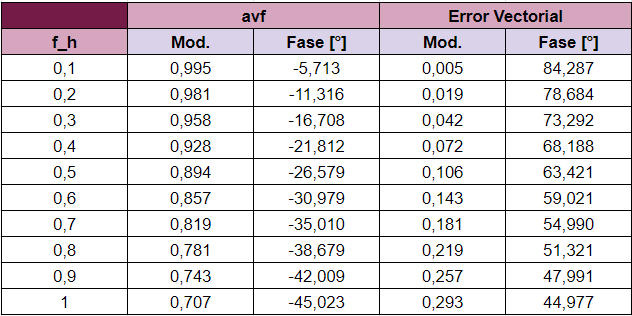
\includegraphics{figuras/lab_2_tabla_ev.png}
    \caption{Error vectorial}
    \label{fig:enter-label}
\end{figure}


%\newpage

\subsection{Simulaciones.}
\onehalfspacing
A continuación se adjuntan las simulaciones para el circuito bajo estudio

\begin{figure}[h!]
    \centering
    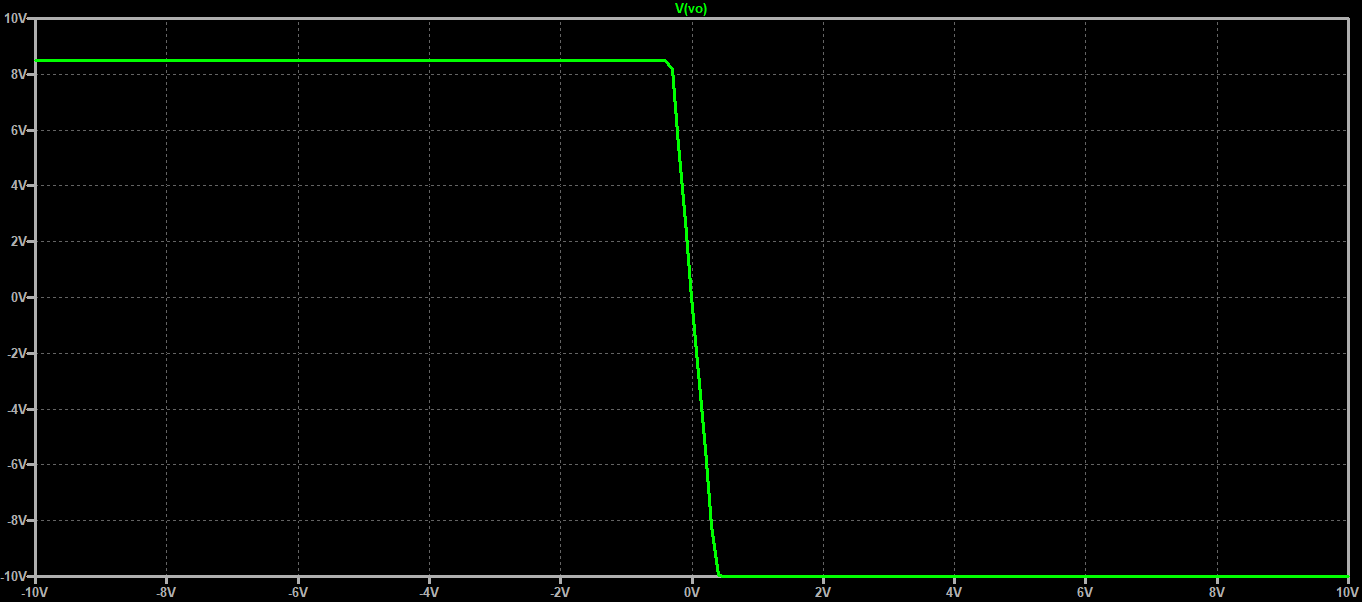
\includegraphics[scale=0.4]{figuras/simulacion1/barrido_-10V_10V_continua.png}
    \caption{Barrido en frecuencia}
    \label{fig:enter-label}
\end{figure}

\begin{figure}[h!]
    \centering
    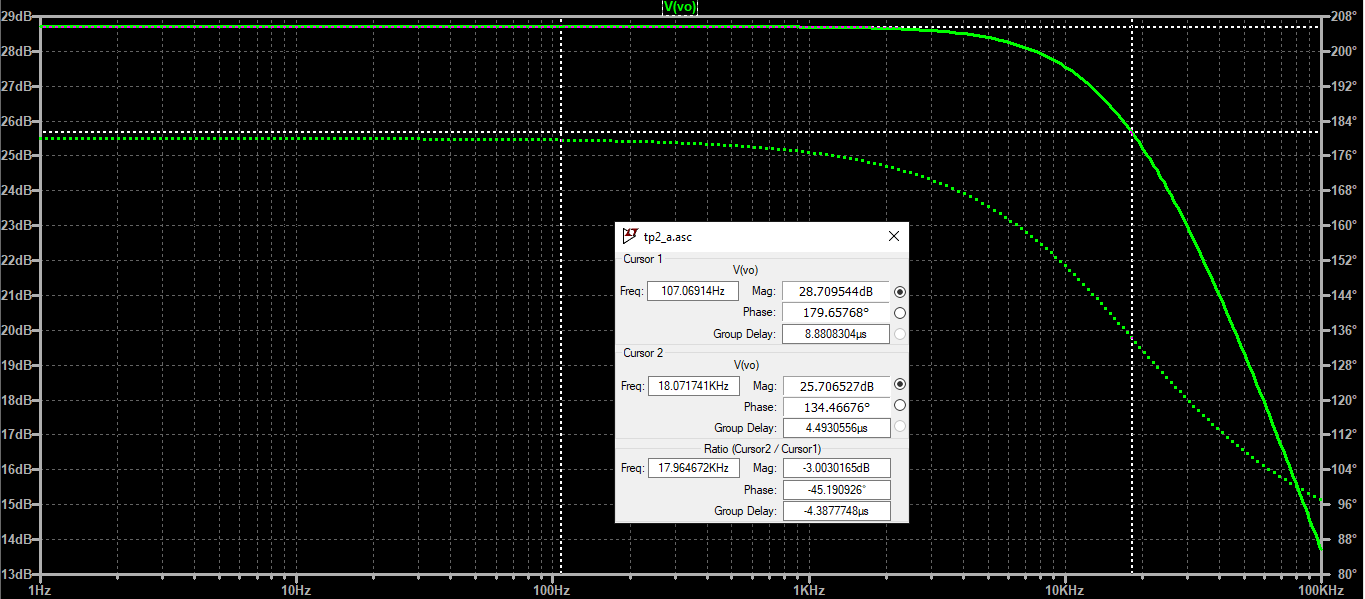
\includegraphics[scale=0.4]{figuras/simulacion1/bode.png}
    \caption{Diagrama de Bode}
    \label{fig:enter-label}
\end{figure}

\begin{figure}[h!]
    \centering
    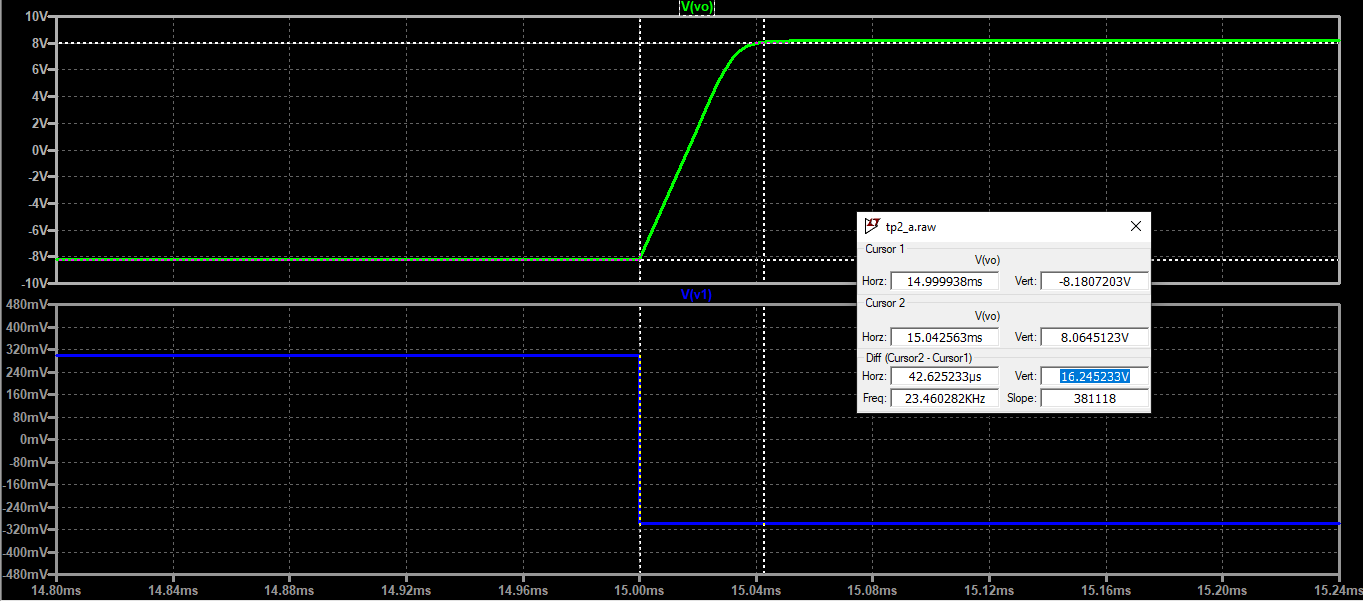
\includegraphics[scale=0.4]{figuras/simulacion1/Slew_Rate_Vin=600mV_PP.png}
    \caption{Slew Rate}
    \label{fig:enter-label}
\end{figure}

\begin{figure}[h!]
    \centering
    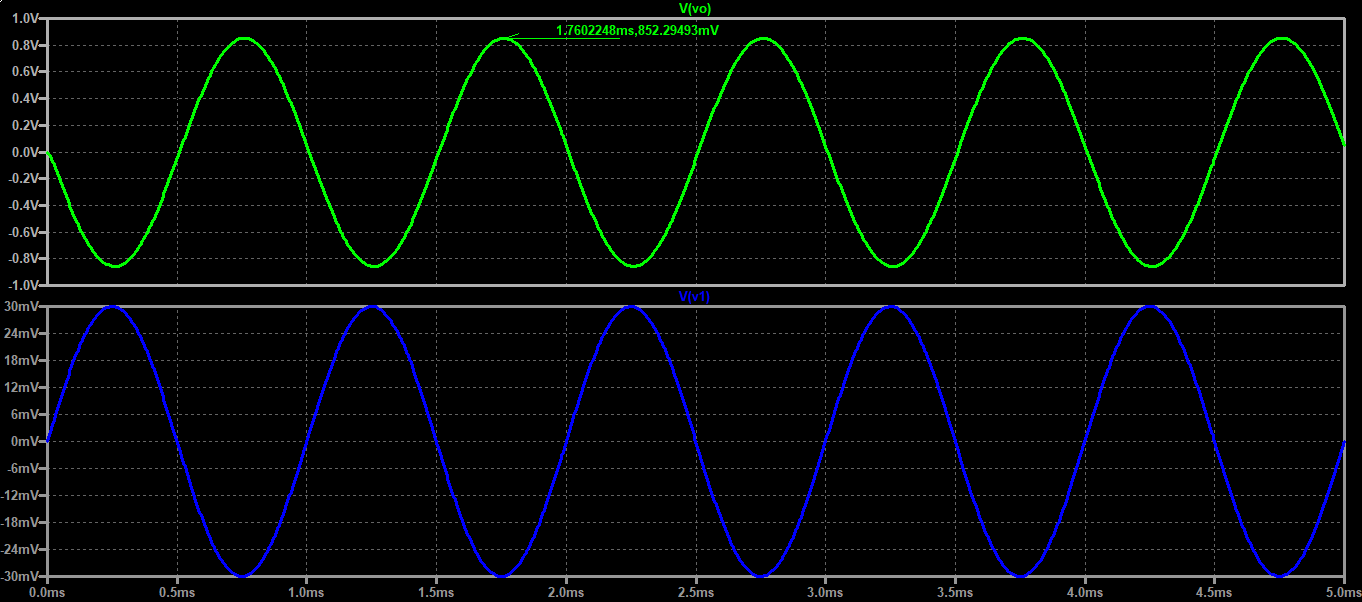
\includegraphics[scale=0.4]{figuras/simulacion1/Vo_Vin=30mV_CA_Ri=50.png}
    \caption{Factor de amplificación, $A_v = 30$}
    \label{fig:enter-label}
\end{figure}

\begin{figure}[h!]
    \centering
    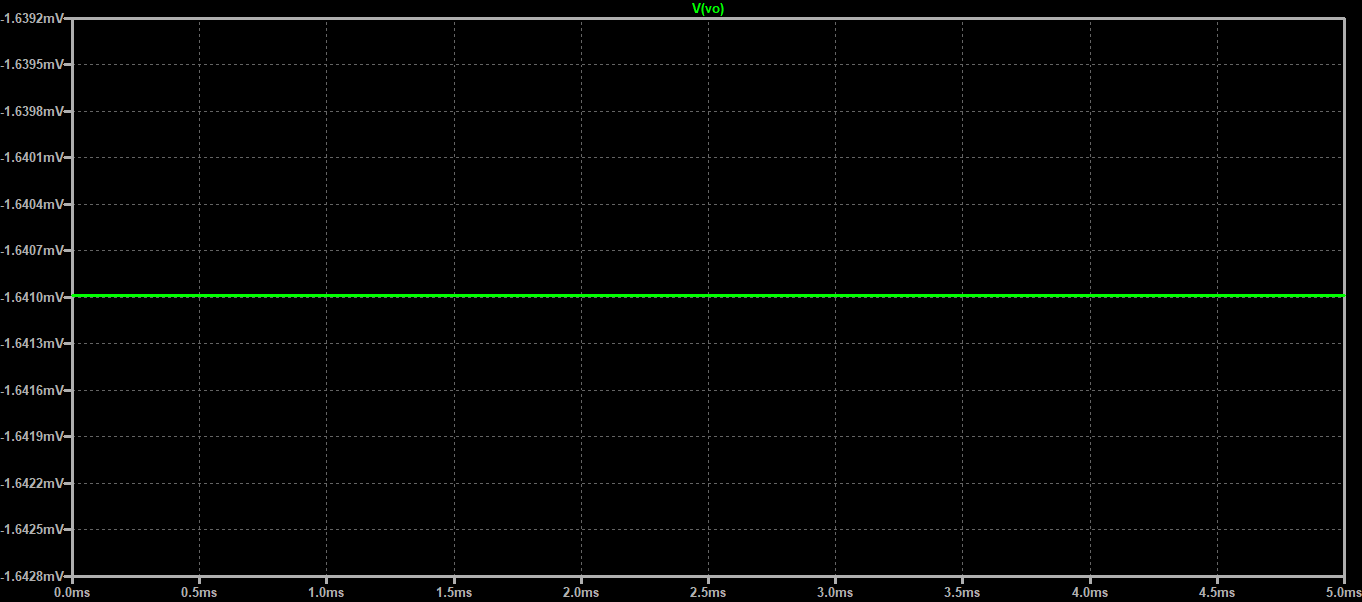
\includegraphics[scale=0.4]{figuras/simulacion1/Vo_Ios_CC.png}
    \caption{Vout(Ios)}
    \label{fig:enter-label}
\end{figure}

\begin{figure}[h!]
    \centering
    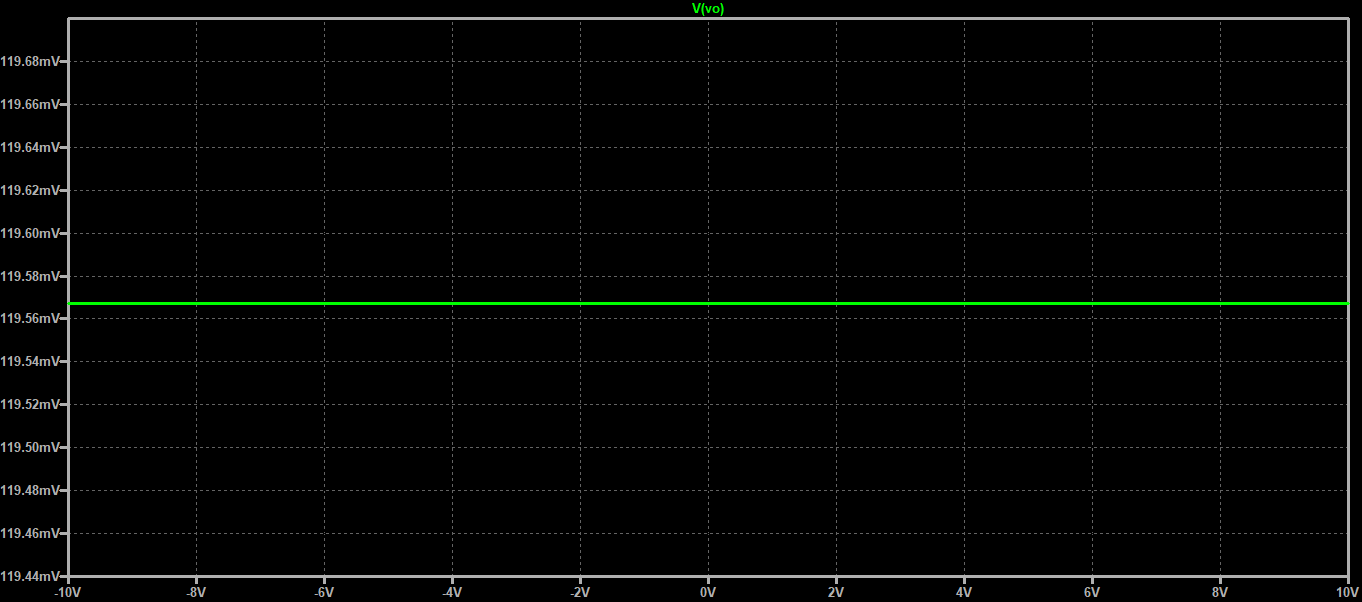
\includegraphics[scale=0.4]{figuras/simulacion1/Vo_Vos=2mV_CC.png}
    \caption{Vout(Vos)}
    \label{fig:enter-label}
\end{figure}

\newpage

\subsection{Implementación.}
\onehalfspacing
Se llevó a cabo la implementación física del circuito analizando la amplificación ofrecida por el mismo, el slew rate y alguno de los errores que fueron posibles de medir con el instrumental disponible.

\begin{figure}[h!]
    \centering
    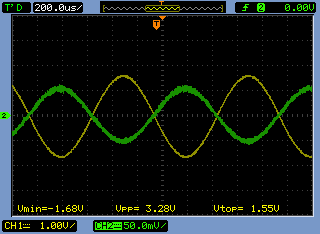
\includegraphics[scale=0.6]{figuras/Implementacion1/NewFile22.png}
    \caption{Factor de ganancia, $V1 = 50mV$}
    \label{fig:enter-label}
\end{figure}

\begin{figure}[h!]
    \centering
    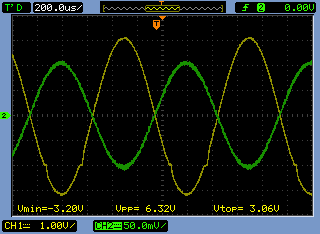
\includegraphics[scale=0.6]{figuras/Implementacion1/NewFile23.png}
    \caption{Factor de ganancia, V1 = 100mV}
    \label{fig:enter-label}
\end{figure}

\begin{figure}[h!]
    \centering
    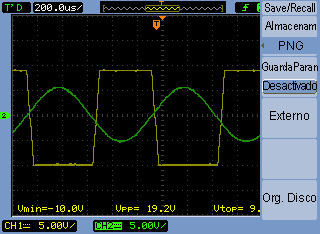
\includegraphics[scale=0.6]{figuras/Implementacion1/NewFile24.png}
    \caption{Factor de ganancia, $V1 = 5V$}
    \label{fig:enter-label}
\end{figure}

\newpage

\begin{figure}[h!]
    \centering
    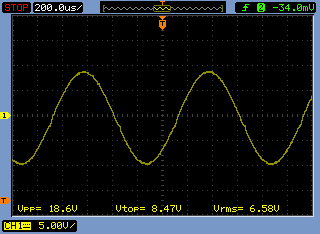
\includegraphics[scale=0.6]{figuras/Implementacion1/NewFile25.png}
    \caption{$Vo=f(Ad  < \infty)$, $V1=333mV$, $V2=0V$}
    \label{fig:enter-label}
\end{figure}

\begin{figure}[h!]
    \centering
    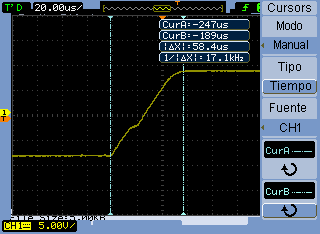
\includegraphics[scale=0.6]{figuras/Implementacion1/NewFile26.png}
    \caption{SR, $V1=320mV$, $f=2kHz$}
    \label{fig:enter-label}
\end{figure}


